\documentclass[11pt,a4paper]{article}
\usepackage{amsmath}
\usepackage{amsfonts}
\usepackage{tikz,pgfplots}
\usepackage{gensymb}
\usepackage{graphicx}

\usepackage{epstopdf}
%\usepackage{listings}
\usepackage{tikz,fp,fp-random,todonotes}
\usepackage[procnames]{listings}
\usepackage{afterpage}
%\usepackage[margin=1in]{geometry}
\usepackage{titlesec}
\usepackage{float}
\usepackage{amsthm}
\usepackage{wrapfig}
\usepackage{booktabs,caption}
\usepackage[flushleft]{threeparttable}
\usepackage{scrextend}
\usepackage{stfloats}
\usepackage{mathtools}
\usepackage{bm}
\usepackage{stackengine}
\usepackage[hidelinks]{hyperref}
\usepackage{siunitx}
\usepackage{subfig}
\usepackage{authblk}
\usepackage[margin=0.7in]{geometry}
 
\addtokomafont{labelinglabel}{\sffamily}


\usetikzlibrary{calc}
\usetikzlibrary{backgrounds}
\usetikzlibrary{calc}
\usetikzlibrary{decorations.markings}
\usetikzlibrary{arrows}
\usetikzlibrary{positioning}
\usetikzlibrary{decorations.text}

\usetikzlibrary{shadings}
\usetikzlibrary{backgrounds}
\usetikzlibrary{calc}
\usetikzlibrary{decorations.markings}
\usetikzlibrary{arrows}
\usetikzlibrary{positioning}
\usetikzlibrary{decorations.text}
        
\allowdisplaybreaks
\renewcommand{\floatpagefraction}{.85}

\newcommand{\x}{{\bf x}}
\renewcommand{\d}{{\rm d}}
\newcommand{\e}{{\rm e}}
\newcommand{\ii}{{\rm i}}

\newcommand{\tmi}{\tau_0\wedge\tau}
\newcommand{\tma}{\tau_0\vee\tau}
\newcommand{\taua}{\tau_{\rm A}}


\begin{document}
\title{Evolutionary rescue}
\author[1]{Remus Stana}
\author[1]{Yoav Ram}
\author[2]{‪Daniel Weissman}
\affil[1]{School of Zoology, Tel Aviv University, Tel Aviv-Yafo, Israel}
\affil[2]{Department of Physics, Emory University, Atlanta, United States of America}
\maketitle
\begin{abstract}
\end{abstract}

\section{Introduction}
The question of what role does chromosomal instability (CIN) play in the emergence of cancer has been studied extensively in the past decades \cite{michor2005can,christine2018understanding,nowak2002role,pavelka2010dr,komarova2003mutation,zhu2018cellular}. One hypothesis is that CIN facilitates tumorgenesis by accelerating the removal of tumor suppression genes (TSG) and subsequent appearance of cancer. The deletion of tumor suppression genes can happen in two ways (see Figure \ref{figureCIN}): two point mutations deleting both alleles of the TSG or one point mutation and one chromosomal loss event. The case of two chromosomal loss events is taken into consideration because the fitness cost would be very large and the cell would die.

Populations adapted to a certain environment are vulnerable to change in the environment which might cause extinction of the population. Adaptation is a race against time as the population size decreases in the new environment. Evolutionary rescue is the process where the population acquires mutations which increases the fitness of the population in the new environment such that the extinction in averted. We are interested in how likely is a population to adapt to the changing environment through evolution. Examples of such changes include climate change, invasive species or the onset of drug therapies. There exists three possible ways for a population to survive environmental degradation: migration to a new habitat similar to the one before the onset of environmental changes \cite{cobbold2020should}, adaptation by phenotypic plasticity which involves no changes in the genotype\cite{carja2019evolutionary,carja2017evolutionary} and adaptation through genetic mutations\cite{uecker2014evolutionary,uecker2016role,uecker2011fixation}.

Majority of studies assume that the fitness of the wildtype and mutant are time homogeneous. An exception is \cite{marrec2020adapt} fitness of wildtype and mutant are taken to be functions of time.

\begin{figure}
\centering
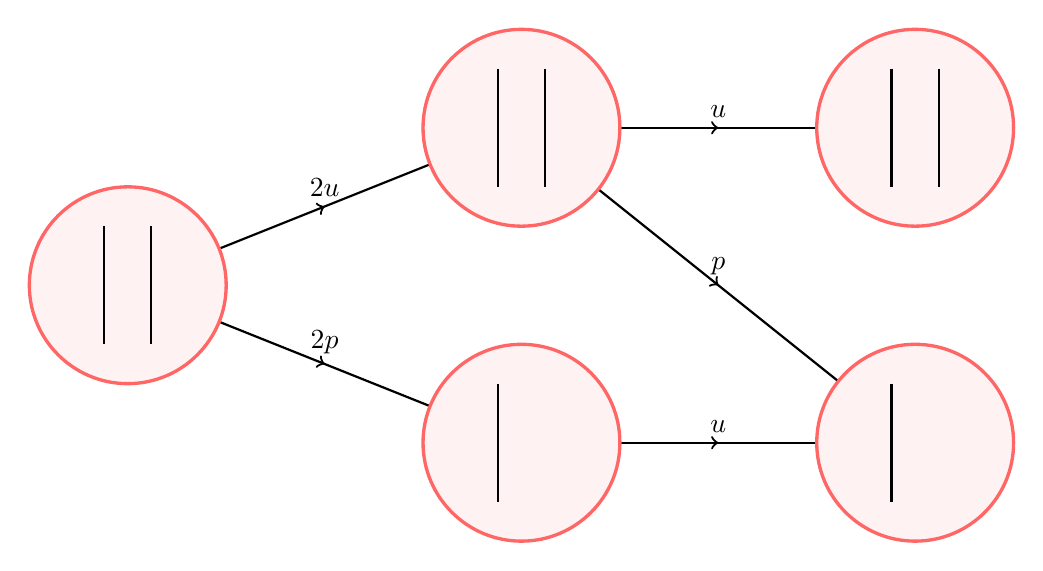
\begin{tikzpicture}[very thick,decoration={
    markings,
    mark=at position 0.5 with {\arrow{>}}}
    ] 
\edef\x{6.5} 
\edef\y{-0.5} 
\edef\r{1.25} 

\draw [postaction={decorate}, thick](-0.25,-2) -- (-0.25+5,0) node [midway, above] {$2u$};
\draw [postaction={decorate}, thick](-0.25,-2) -- (-0.25+5,-4) node [midway, above] {$2p$};
\draw [postaction={decorate}, thick](-0.25+5+\r,-0) -- (-0.25+10-\r,-0) node [midway, above] {$u$};
\draw [postaction={decorate}, thick](-0.25+5+\r,-4) -- (-0.25+10-\r,-4) node [midway, above] {$u$};
\draw [postaction={decorate}, thick](-0.25+5,-0) -- (-0.25+10,-4) node [midway, above] {$p$};

\filldraw[color=red!60, fill=red!5, very thick](-0.25,-2) circle (\r);
\filldraw[color=red!60, fill=red!5, very thick](-0.25+5,0) circle (\r);
\filldraw[color=red!60, fill=red!5, very thick](-0.25+5,-4) circle (\r);
\filldraw[color=red!60, fill=red!5, very thick](-0.25+10,0) circle (\r);
\filldraw[color=red!60, fill=red!5, very thick](-0.25+10,-4) circle (\r);

\draw [thick](0.05,-1.25) -- (0.05,-2.75);
\draw [thick](-0.55,-1.25) -- (-0.55,-2.75);

\draw [thick](0.05+5,-1.25+2) -- (0.05+5,-2.75+2);
\draw [thick](-0.55+5,-1.25+2) -- (-0.55+5,-2.75+2);

\draw [thick](0.05+10,-1.25+2) -- (0.05+10,-2.75+2);
\draw [thick](-0.55+10,-1.25+2) -- (-0.55+10,-2.75+2);

\draw [thick](-0.55+5,-1.25-2) -- (-0.55+5,-2.75-2);

\draw [thick](-0.55+10,-1.25-2) -- (-0.55+10,-2.75-2);
\end{tikzpicture}
\caption{
}
\label{figureCIN}
\end{figure}

\section{Model}
We model evolutionary rescue of cancer cells through aneuploidy with the help of multitype branching processes: we have three populations of cancer cells, wildtype, aneuploidy and mutant cells which proliferate and die with rates $\lambda_w,  \lambda_a,  \lambda_m$ and $\mu_w, \mu_a, \mu_m$, respectively. Wildtype cells can acquire aneuploidy at rate $u$ while aneuploidy and wildtype cells can mutate with rate $v$ (se Figure \ref{figureAneuploidy}). The probability that a single mutant cell will survive is given by\cite{allen2010introduction}:
\begin{equation}
p_m=\left\{
  \begin{array}{@{}ll@{}}
  \frac{\lambda_m-\mu_m}{\lambda_m},\quad\text{if }\lambda_m>\mu_m \\
   0,\quad\text{else}.
  \end{array}\right.
  \end{equation}
 If the population originally consists of a single aneuploidy cell, then the probability that the population will survive is given by the following quadratic equation:
\begin{align}
1-p_a=\frac{\mu_a}{\lambda_a+\mu_a+v}+\frac{v}{\lambda_a+\mu_a+v}\left(1-p_m\right)+\frac{\lambda_a}{\lambda_a+\mu_a+v}\left(1-p_a\right)^2,
\end{align}
whose smallest solution is the survival probability:
\begin{align}\label{survproba}
p_a=\frac{\lambda_a-\mu_a-v+\sqrt{\left(\lambda_a-\mu_a-v\right)^2+4\lambda_avp_m}}{2\lambda_a}.
\end{align}
Analogously, the survival probability of a population consisting initially of one wildtype cell satisfies the quadratic equation:
\begin{align}\nonumber
1-p_w&=\frac{\mu_w}{\lambda_w+\mu_w+u+v}+\frac{u}{\lambda_w+\mu_w+u+v}\left(1-p_a\right)+\frac{\lambda_w}{\lambda_w+\mu_w+u+v}\left(1-p_w\right)^2\\
&+\frac{v}{\lambda_w+\mu_w+u+v}\left(1-p_m\right),
\end{align}
where the smallest solution gives the survival probability:
\begin{align}\label{survprobw}
p_w=\frac{\lambda_w-\mu_w-u-v+\sqrt{\left(\lambda_w-\mu_w-u-v\right)^2+4\lambda_w\left(up_a+vp_m\right)}}{2\lambda_w}.
\end{align}

%%%%%%%%%%%%%%%%%%%%%%%%%%%%%%%%%%%%%%%%%%%%%%%%%%%%%%%%%%%%
\begin{figure}
\centering
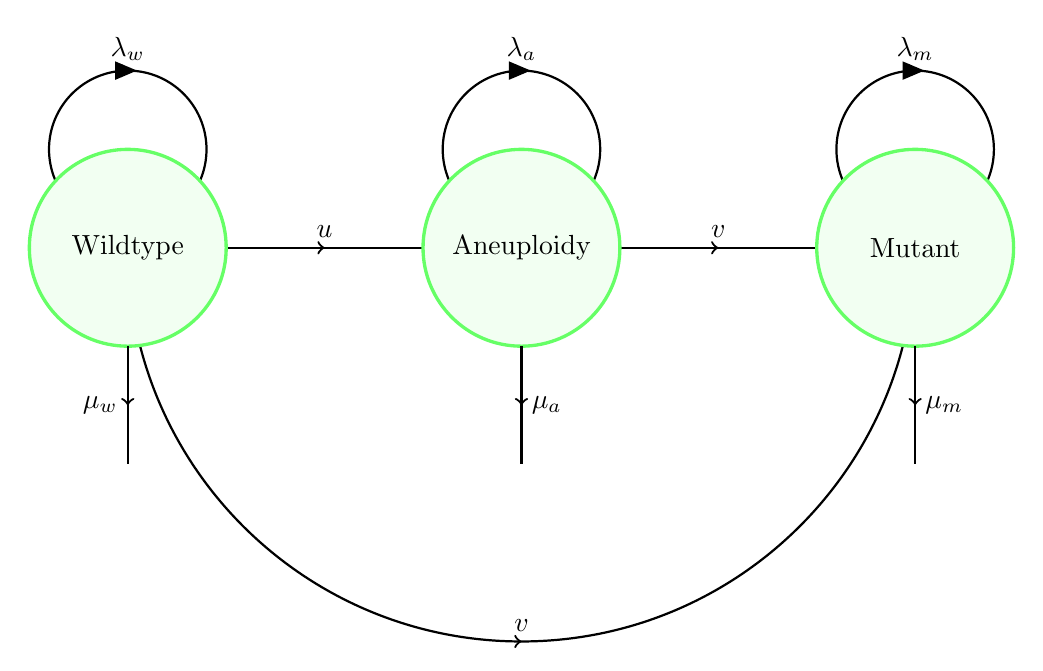
\begin{tikzpicture}[very thick,decoration={
    markings,
    mark=at position 0.5 with {\arrow{>}}}, middlearrow/.style 2 args={
        decoration={             
            markings, 
            mark=at position 0.5 with {\arrow[xshift=3.333pt]{triangle 45}, \node[#1] {#2};}
        },
        postaction={decorate}
    }]
\edef\x{6.5} 
\edef\y{-0.5} 
\edef\r{1.25} 

\edef\R{1} 
\edef\Y{0.25} 

\draw[black,thick,middlearrow={above}{$\lambda_w$},text=black] (-0.25,\Y) arc (270:-90:\R);
\draw[black,thick,middlearrow={above}{$\lambda_a$},text=black] (-0.25+5,\Y) arc (270:-90:\R);
\draw[black,thick,middlearrow={above}{$\lambda_m$},text=black] (-0.25+10,\Y) arc (270:-90:\R);

\draw [postaction={decorate}, thick](-0.25,0) -- (-0.25+5,0) node [midway, above] {$u$};
\draw [postaction={decorate}, thick](-0.25+5+\r,-0) -- (-0.25+10-\r,-0) node [midway, above] {$v$};

\draw[thick, postaction={decorate}] (-0.25,0) arc (180:360:5) node [midway, above] {$v$};


\filldraw[color=green!60, fill=green!5, very thick](-0.25,0) circle (\r);
\filldraw[color=green!60, fill=green!5, very thick](-0.25+5,0) circle (\r);
\filldraw[color=green!60, fill=green!5, very thick](-0.25+10,0) circle (\r);

\draw [thick, postaction={decorate}](-0.25,-1.25) -- (-0.25,-2.75) node [midway, left] {$\mu_w$};

\draw [thick, postaction={decorate}](-0.25+5,-1.25) -- (-0.25+5,-2.75) node [midway, right] {$\mu_a$};

\draw [thick, postaction={decorate}](-0.25+10,-1.25) -- (-0.25+10,-2.75) node [midway, right] {$\mu_m$};

\edef\y{-0.25} 

\node at (\y,0) {Wildtype};
\node at (\y+5,0) {Aneuploidy};
\node at (\y+10,0) {Mutant};
\end{tikzpicture}
\caption{Diagram of the evolutionary rescue model where the population of cancer cells is subdivided into three populations of cancer cells, wildtype, aneuploidy and mutant cells which proliferate and die with rates $\lambda_w,  \lambda_a,  \lambda_m$ and $\mu_w, \mu_a, \mu_m$, respectively. Wildtype cells can acquire aneuploidy at rate $u$ while aneuploidy and wildtype cells can mutate with rate $v$.}
\label{figureAneuploidy}
\end{figure}
%%%%%%%%%%%%%%%%%%%%%%%%%%%%%%%%%%%%%%%%%%%%%%%%%%%%%%%%%%%%%

\section{First case: $4\lambda_avp_m<\left(\lambda_a-\mu_a-v\right)^2$}
We assume that $\mu_w>\lambda_w$ and $\mu_a<\lambda_a$ and, as a result, we rewrite \eqref{survproba} and \eqref{survprobw} as:
\begin{align*}
p_a&=\frac{\lambda_a-\mu_a-v}{2\lambda_a}\left(1+\sqrt{1+\frac{4\lambda_avp_m}{\left(\lambda_a-\mu_a-v\right)^2}}\right),\\
p_w&=\frac{\lambda_w-\mu_w-u-v}{2\lambda_w}\left(1-\sqrt{1+\frac{4\lambda_w\left(vp_m+up_a\right)}{\left(\lambda_w-\mu_w-u-v\right)^2}}\right).
\end{align*}
Making use of the Taylor series expansions:
\begin{align*}
\left(1+\frac{4\lambda_avp_m}{\left(\lambda_a-\mu_a-v\right)^2}\right)^{\frac{1}{2}}&=1+\frac{2\lambda_avp_m}{\left(\lambda_a-\mu_a-v\right)^2}+\cdots\\
\left(1+\frac{4\lambda_w\left(vp_m+up_a\right)}{\left(\lambda_w-\mu_w-u-v\right)^2}\right)^{\frac{1}{2}}&=1+\frac{2\lambda_w\left(vp_m+up_a\right)}{\left(\lambda_a-\mu_a-u-v\right)^2}+\cdots
\end{align*}
we obtain the following approximation for the survival probability of a population consisting of a single individual wildtype cell:
\begin{align}\label{survprobwinitial}
p_w&\approx\frac{vp_m+up_a}{\lambda_a-\mu_a-u-v}\\
\nonumber
&\approx-\frac{1}{\lambda_w-\mu_w-u-v}\left[\frac{v\left(\lambda_a-\mu_a-u\right)}{\lambda_a}+\frac{uv\left(\lambda_m-\mu_m\right)}{\lambda_m\left(\lambda_a-\mu_a-u\right)}+\frac{v\left(\lambda_m-\mu_m\right)}{\lambda_m}\right]\\ \label{survprobw}
&\approx-\frac{1}{\lambda_w-\mu_w-u-v}\left[\frac{v\left(\lambda_a-\mu_a\right)}{\lambda_a}+\frac{uv\left(\lambda_m-\mu_m\right)}{\lambda_m\left(\lambda_a-\mu_a\right)}+\frac{v\left(\lambda_m-\mu_m\right)}{\lambda_m}\right],
\end{align}
where in the last line we have used the fact that $u,v\ll1$. Using the notational convention
\begin{equation}\label{notationalconv}
\Delta_i=\lambda_i-\mu_i,
\end{equation}
we write \eqref{survprobw} as
\begin{equation}\label{survprobwapprox}
p_w=-\frac{1}{\Delta_w}\left(\frac{v\Delta_a}{\lambda_a}+\frac{uv\Delta_m}{\lambda_m\Delta_a}+\frac{v\Delta_m}{\lambda_m}\right).
\end{equation}
Given an initial population consisting of $N$ wildtype cancer cells, the probability that the population will survive is given by: 
\begin{align}
p_{est}=1-\left(1-p_w\right)^N\approx 1-\e^{-Np_w}=1-\exp\left[\frac{N}{\Delta_w}\left(\frac{v\Delta_a}{\lambda_a}+\frac{uv\Delta_m}{\lambda_m\Delta_a}+\frac{v\Delta_m}{\lambda_m}\right)\right],
\end{align}
which we plot in Figure \ref{SurvPlotNData} as a function of $N$ and in Figure \ref{SurvPlot} as a function of $\lambda_w$. 

We want to improve the accuracy of our approximation by taking into consideration the second term of the Taylor series expansion:
\begin{align*}
\left(1+\frac{4\lambda_avp_m}{\left(\lambda_a-\mu_a-v\right)^2}\right)^{\frac{1}{2}}=1+\frac{2\lambda_avp_m}{\left(\lambda_a-\mu_a-v\right)^2}-\frac{\left(\lambda_avp_m\right)^2}{4\left(\lambda_a-\mu_a-v\right)^4}+\cdots,
\end{align*}
which gives us the following approximation for $p_a$:
\begin{align}
p_a=\frac{\lambda_a-\mu_a-v}{\lambda_a}+\frac{vp_m}{\lambda_a-\mu_a-v}-\frac{\lambda_a\left(vp_m\right)^2}{8\left(\lambda_a-\mu_a-v\right)^3}
\end{align}
From which we deduce that:
\begin{align}\nonumber
p_w&\approx-\frac{1}{\lambda_w-\mu_w-u-v}\left[\frac{v\left(\lambda_a-\mu_a-u\right)}{\lambda_a}+\frac{uv\left(\lambda_m-\mu_m\right)}{\lambda_m\left(\lambda_a-\mu_a-u\right)}+\frac{v\left(\lambda_m-\mu_m\right)}{\lambda_m}-\frac{uv^2\lambda_a\left(\lambda_m-\mu_m\right)^2}{8\lambda_m^2\left(\lambda_a-\mu_a-v\right)^3}\right]\\ \label{survprobw}
&\approx-\frac{1}{\lambda_w-\mu_w-u-v}\left[\frac{v\left(\lambda_a-\mu_a\right)}{\lambda_a}+\frac{uv\left(\lambda_m-\mu_m\right)}{\lambda_m\left(\lambda_a-\mu_a\right)}+\frac{v\left(\lambda_m-\mu_m\right)}{\lambda_m}-\frac{uv^2\lambda_a\left(\lambda_m-\mu_m\right)^2}{8\lambda_m^2\left(\lambda_a-\mu_a\right)^3}\right].
\end{align}
Using the notations described in \eqref{notationalconv} we write the above equation as:
\begin{equation}\label{survprobwapproxcorrected}
p_w=-\frac{1}{\Delta_w}\left(\frac{v\Delta_a}{\lambda_a}+\frac{uv\Delta_m}{\lambda_m\Delta_a}+\frac{v\Delta_m}{\lambda_m}-\frac{uv^2\lambda_a\Delta_m^2}{8\lambda_m^2\Delta_a^3}\right).
\end{equation}
Given an initial population consisting of $N$ wildtype cancer cells, the probability that the population will survive is given by: 
\begin{align}
p_{est}=1-\left(1-p_w\right)^N\approx 1-\e^{-Np_w}=1-\exp\left[\frac{N}{\Delta_w}\left(\frac{v\Delta_a}{\lambda_a}+\frac{uv\Delta_m}{\lambda_m\Delta_a}+\frac{v\Delta_m}{\lambda_m}\right)\right].
\end{align}
\section{Second case: $4\lambda_avp_m>\left(\lambda_a-\mu_a-v\right)^2$}
If we assume that  $4\lambda_avp_m>\left(\lambda_a-\mu_a-v\right)^2$ then we write:
\begin{equation}
p_a=\frac{\lambda_a-\mu_a-v+2\sqrt{\lambda_a vp_m}\left(1+\frac{\left(\lambda_a-\mu_a-v\right)^2}{4\lambda_avp_m}\right)^{\frac12}}{2\lambda_a}
\end{equation}
and using the following Taylor series expansion:
\begin{align*}
\left(1+\frac{\left(\lambda_a-\mu_a-v\right)^2}{4\lambda_avp_m}\right)^{\frac{1}{2}}=1+\frac{\left(\lambda_a-\mu_a-v\right)^2}{8\lambda_avp_m}+\cdots
\end{align*}
we obtain:
\begin{align*}
p_a&\approx\frac{\lambda_a-\mu_a-v+2\sqrt{\lambda_a vp_m}\left[1+\frac{\left(\lambda_a-\mu_a-v\right)^2}{8\lambda_avp_m}\right]}{2\lambda_a}\\
&=\frac{\lambda_a-\mu_a-v+2\sqrt{\lambda_a vp_m}+\frac{\left(\lambda_a-\mu_a-v\right)^2}{4\sqrt{\lambda_avp_m}}}{2\lambda_a}\\
&\approx\sqrt{\frac{v\left(\lambda_m-\mu_m\right)}{\lambda_a\lambda_m}}
\end{align*}
In the last line of the above we have used the following inequalities:
\begin{align*}
\lambda_a-\mu_a,\,v,\,\frac{\left(\lambda_a-\mu_a-v\right)^2}{4\sqrt{\lambda_avp_m}}\ll1.
\end{align*}
As a result, we have from \eqref{survprobwinitial} the probability of rescue of a population starting from one wildtype individual:
\begin{align*}
p_w&\approx\frac{1}{\lambda_a-\mu_a-u-v}\left[v\frac{\lambda_m-\mu_m}{\lambda_m}+u\sqrt{\frac{v\left(\lambda_m-\mu_m\right)}{\lambda_a\lambda_m}}\right]\\
&=\sqrt{\frac{\lambda_m-\mu_m}{\lambda_m}}\frac{\sqrt{v}}{\lambda_a-\mu_a-u-v}\left[\frac{u}{\sqrt{\lambda_a}}+\sqrt{\frac{v\left(\lambda_m-\mu_m\right)}{\lambda_m}}\right]\\
&=\sqrt{\frac{\Delta_m}{\lambda_m}}\frac{\sqrt{v}}{\Delta_a-u-v}\left[\frac{u}{\sqrt{\lambda_a}}+\sqrt{\frac{v\Delta_m}{\lambda_m}}\right],
\end{align*}
where in the last line we have used the notations defined in \eqref{notationalconv}.

Given an initial population consisting of $N$ wildtype cancer cells, the probability that the population will survive is given by: 
\begin{align*}
p_{est}=1-\left(1-p_w\right)^N\approx 1-\e^{-Np_w}=1-\exp\left[-N\sqrt{\frac{\Delta_m}{\lambda_m}}\frac{\sqrt{v}}{\Delta_a-u-v}\left(\frac{u}{\sqrt{\lambda_a}}+\sqrt{\frac{v\Delta_m}{\lambda_m}}\right)\right].
\end{align*}


\section{Standing genetic variation}
Until now we have assumed that the initial population of cells consisted entirely of wildtype cells. We modify this assumtion such that the initial population includes a fraction $f$ of cells with aneuploidy. The probability of evolutionary rescue by the cells with aneuploidy from the initial population is:
\begin{equation*}
p_{old}=1-\left(1-p_a\right)^{fN}\approx 1-\e^{-fNp_a}.
\end{equation*}
The total probability of evolutionary rescue is given by:
\begin{align}\nonumber
p_{total}&=p_{new}+\left(1-p_{new}\right)p_{old}\\
&=1-\e^{-\left[\left(1-f\right)p_w+fp_a\right]N}.
\end{align}
The fraction of the cases in which the population is rescued by the standing genetic variation is given by:
\begin{align*}
F\left(f\right)=\frac{ 1-\e^{-fNp_a}}{1-\e^{-\left[\left(1-f\right)p_w+fp_a\right]N}}.
\end{align*}
We let $F=\frac{1}{2}$ and we obtain:
\begin{equation*}
f^*\approx\frac{p_w}{p_w+p_a},
\end{equation*}
wher we have used the expansion $\e^x\approx 1+x$.
We plot $F$ and $f^*$ in Figure \ref{FractionPlot}.

\section{Discussion}



\begin{figure}[!t]
 \vspace*{1\baselineskip}
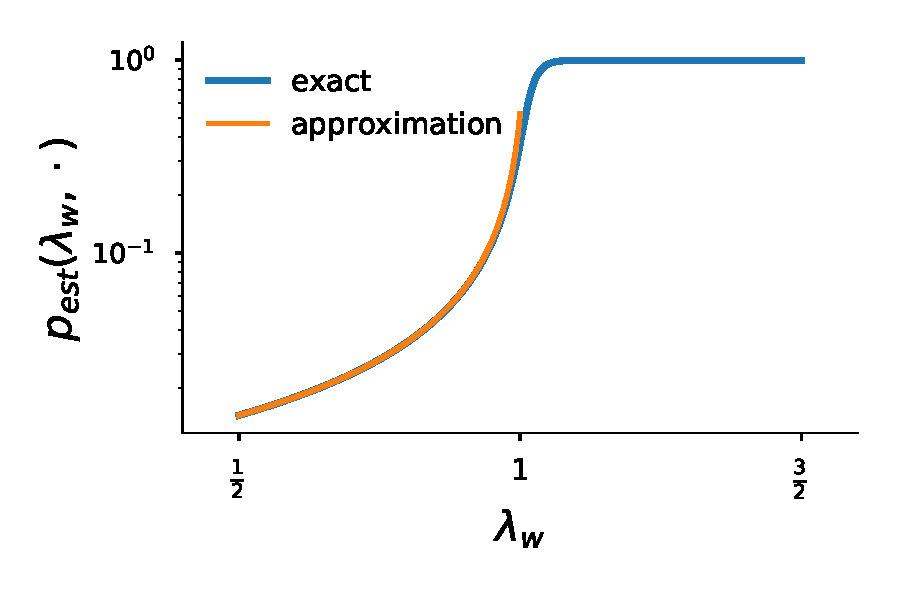
\includegraphics[width=1\textwidth]{SurvPlot.pdf}
\caption{Plot of the probability of survival of a population as a function of the proliferation rate of the wildtype cells. The blue line represents the exact solution \eqref{survprobw} and the orange line line represents the approximation \eqref{survprobwapprox}. Here the population initially consists of $N$ wildtype cells and for the simulations we have chosen the following parameters: $N=75, \lambda_a=1+10^{-2},\lambda_m=1+10^{-3},\mu_w=1,\mu_a=1,\mu_m=1.$}
\label{SurvPlot}
\end{figure}

\begin{figure}[!t]
 \vspace*{1\baselineskip}
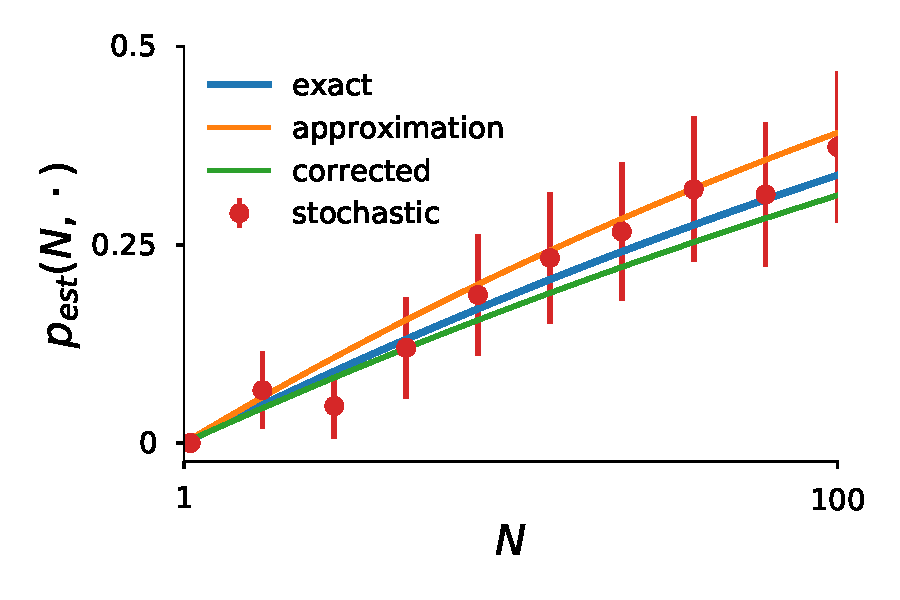
\includegraphics[width=1\textwidth]{SurvPlotNData.pdf}
\caption{Plot of the probability of survival of a population as a function of the initial population size of wildtype cells. The blue line represents the exact solution \eqref{survprobw}, the orange line line represents the approximation \eqref{survprobwapprox}, the green line represents the first order correction \eqref{survprobwapproxcorrected} and the red dots represents stochastic simulations. For the simulations we have chosen the following parameters: $\lambda_w=1-10^{-2}, \lambda_a=1+10^{-2},\lambda_m=1+10^{-3},\mu_w=1,\mu_a=1,\mu_m=1.$}
\label{SurvPlotNData}
\end{figure}

\begin{figure}[!t]
 \vspace*{1\baselineskip}
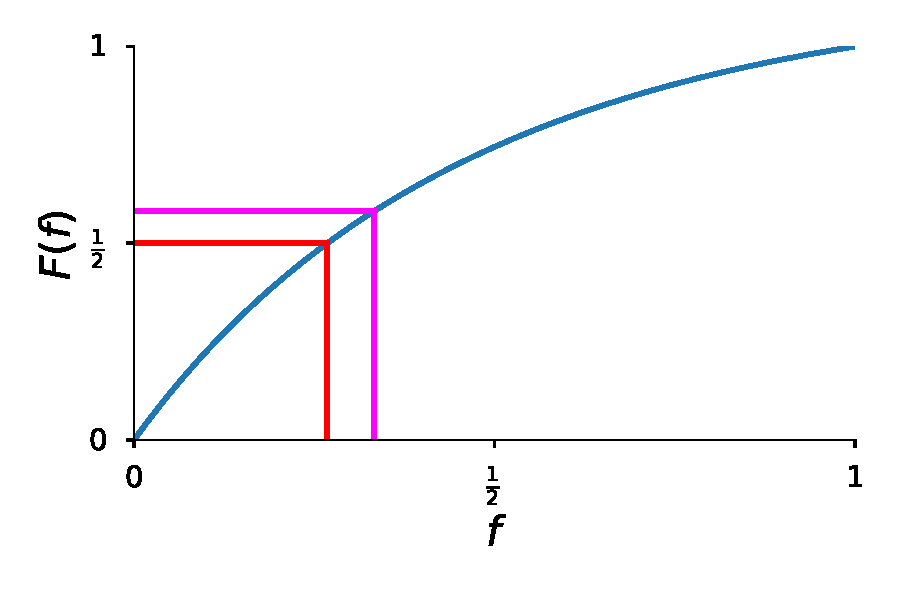
\includegraphics[width=1\textwidth]{FractionPlot.pdf}
\caption{}
\label{FractionPlot}
\end{figure}

\bibliographystyle{unsrt}
\bibliography{green2021}
\end{document}